\documentclass[12pt]{article}
\usepackage[english]{babel}
\usepackage[utf8]{inputenc}

%% Pointer to 'default' preamble, other reusable files
% pacakages and definitions

\usepackage{geometry}
\geometry{
	letterpaper, 
	portrait, 
	top=.75in,
	left=.8in,
	right=.75in,
	bottom=.5in		} 	% Page Margins
	
%% additional packages for nice things
\usepackage{amsmath} 	% for most math
\usepackage{commath} 	% for abs
\usepackage{lastpage}	% for page count
\usepackage{amssymb} 	% for therefore
\usepackage{graphicx} 	% for image handling
\usepackage{wrapfig} 	% wrap figures
\usepackage[none]{hyphenat} % for no hyphenations
\usepackage{array} 		% for >{} column characterisctis
\usepackage{physics} 	% for easier derivative \dv....
\usepackage{tikz} 		% for graphic@!
\usepackage{circuitikz} % for circuits!
\usetikzlibrary{arrows.meta} % for loads
\usepackage[thicklines]{cancel}	% for cancels
\usepackage{xcolor}		% for color cancels
\usepackage[per-mode=fraction]{siunitx} % for si units and num
\sisetup{group-separator = {,}, group-minimum-digits = 3} % additional si unit table functionality

\usepackage{fancyhdr} 	% for header
\usepackage{comment}	% for ability to comment out large sections
\usepackage{multicol}	% for multiple columns using multicols
\usepackage[framed,numbered]{matlab-prettifier} % matlab sytle listing
\usepackage{marvosym} 	% for boltsymbol lightning
\usepackage{pdflscape} 	% for various landscape pages in portrait docs.
%\usepackage{float}
\usepackage{fancyvrb}	% for Verbatim (a tab respecting verbatim)
\usepackage{enumitem}	% for [resume] functionality of enumerate
\usepackage{spreadtab} 	% for using formulas in tables}
\usepackage{numprint}	% for number format in spread tab
\usepackage{subcaption} % for subfigures with captions
\usepackage[normalem]{ulem} % for strike through sout

% for row colors in tables....
\usepackage{color, colortbl}
\definecolor{G1}{gray}{0.9}
\definecolor{G2}{rgb}{1,0.88,1}%{gray}{0.6}
\definecolor{G3}{rgb}{0.88,1,1}

% For table formatting
\usepackage{booktabs}
\renewcommand{\arraystretch}{1.2}
\usepackage{floatrow}
\floatsetup[table]{capposition=top} % put table captions on top of tables

% Caption formating footnotesize ~ 10 pt in a 12 pt document
\usepackage[font={small}]{caption}

%% package config 
\sisetup{output-exponent-marker=\ensuremath{\mathrm{E}}} % for engineer E
\renewcommand{\CancelColor}{\color{red}}	% for color cancels
\lstset{aboveskip=2pt,belowskip=2pt} % for more compact table
%\arraycolsep=1.4pt\def
\setlength{\parindent}{0cm} % Remove indentation from paragraphs
\setlength{\columnsep}{0.5cm}
\lstset{
	style      = Matlab-editor,
	basicstyle = \ttfamily\footnotesize, % if you want to use Courier - not really used?
}
\renewcommand*{\pd}[3][]{\ensuremath{\dfrac{\partial^{#1} #2}{\partial #3}}} % for larger pd fracs
\renewcommand{\real}[1]{\mathbb{R}\left\{ #1 \right\}}	% for REAL symbol
\newcommand{\imag}[1]{\mathbb{I}\left\{ #1 \right\}}	% for IMAG symbol
\definecolor{m}{rgb}{1,0,1}	% for MATLAB matching magenta
	
%% custom macros
\newcommand\numberthis{\addtocounter{equation}{1}\tag{\theequation}} % for simple \numberthis command

\newcommand{\equal}{=} % so circuitikz can have an = in the labels
\newcolumntype{L}[1]{>{\raggedright\let\newline\\\arraybackslash\hspace{0pt}}m{#1}}
\newcolumntype{C}[1]{>{\centering\let\newline\\\arraybackslash\hspace{0pt}}m{#1}}
\newcolumntype{R}[1]{>{\raggedleft\let\newline\\\arraybackslash\hspace{0pt}}m{#1}}

%% Header
\pagestyle{fancy} % for header stuffs
\fancyhf{}
% spacing
\headheight 29 pt
\headsep 6 pt
%%% custom commands for nicer units
\newcommand{\mw}{\ensuremath{\text{ MW}}}
\newcommand{\hz}{\ensuremath{\text{ Hz}}}
\newcommand{\pu}{\ensuremath{\text{ Pu}}}
\newcommand{\sbase}{\ensuremath{\text{S}_{\text{Base}}}}
\newcommand{\fbase}{\ensuremath{f_{\text{Base}}}}
\newcommand{\mbase}[1]{\ensuremath{\text{M}_{\text{Base}_{#1}}}}
\newcommand{\hsys}{\ensuremath{\text{ H}_{\text{sys}}}}


%% Header
\rhead{Thad Haines \\ Page \thepage\ of \pageref{LastPage}}
\chead{MiniWECC \\Step and Trip Results  }
\lhead{Research \\ July 1st, 2019}

\begin{document}
\paragraph{Load Step:}Simulation results with time step = 1.0 second. 1,200 MW Load step at t=2. PSDS must have exciters and PSS models to remain stable.

	\begin{figure}[h!]
			\centering
			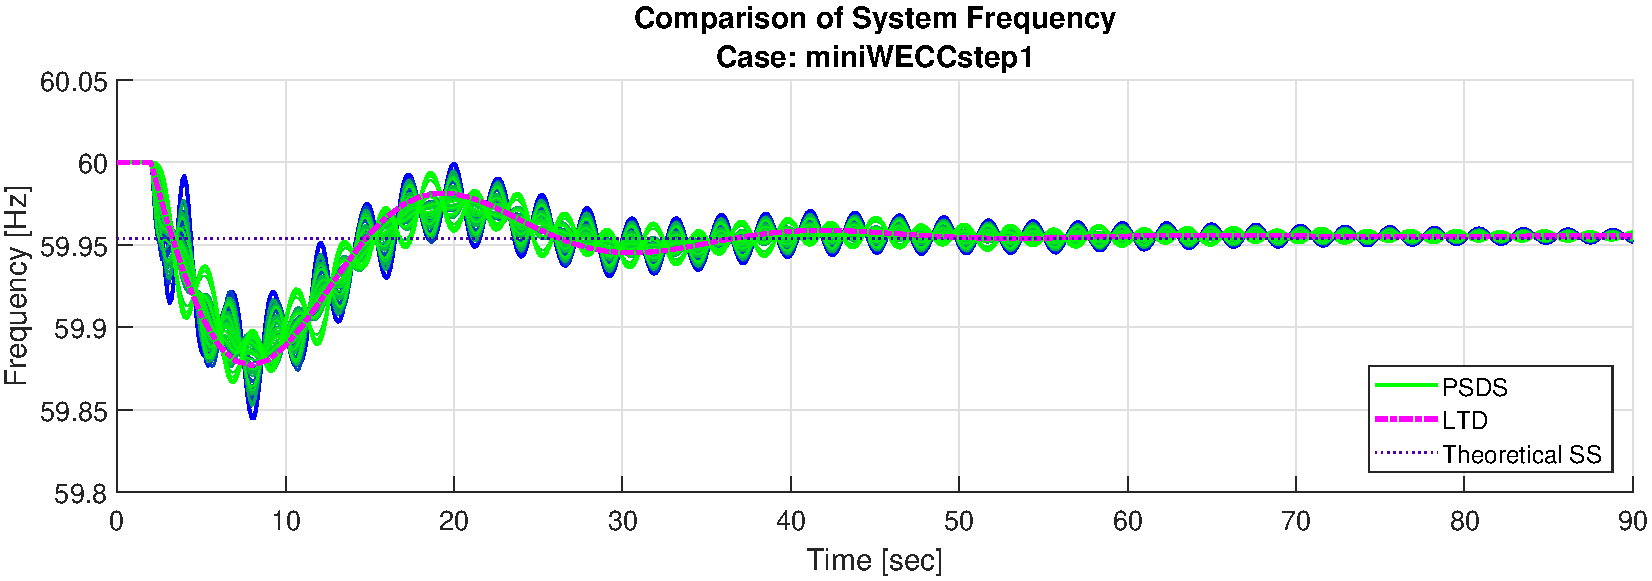
\includegraphics[width=\linewidth]{miniWECCstep1Freq}\vspace{-1em}
			\caption{All PSDS bus frequencies and LTD system frequency response.}
			\label{fcomp}		 
	\end{figure}\vspace{-2em}
	\begin{figure}[h!]
				\centering
				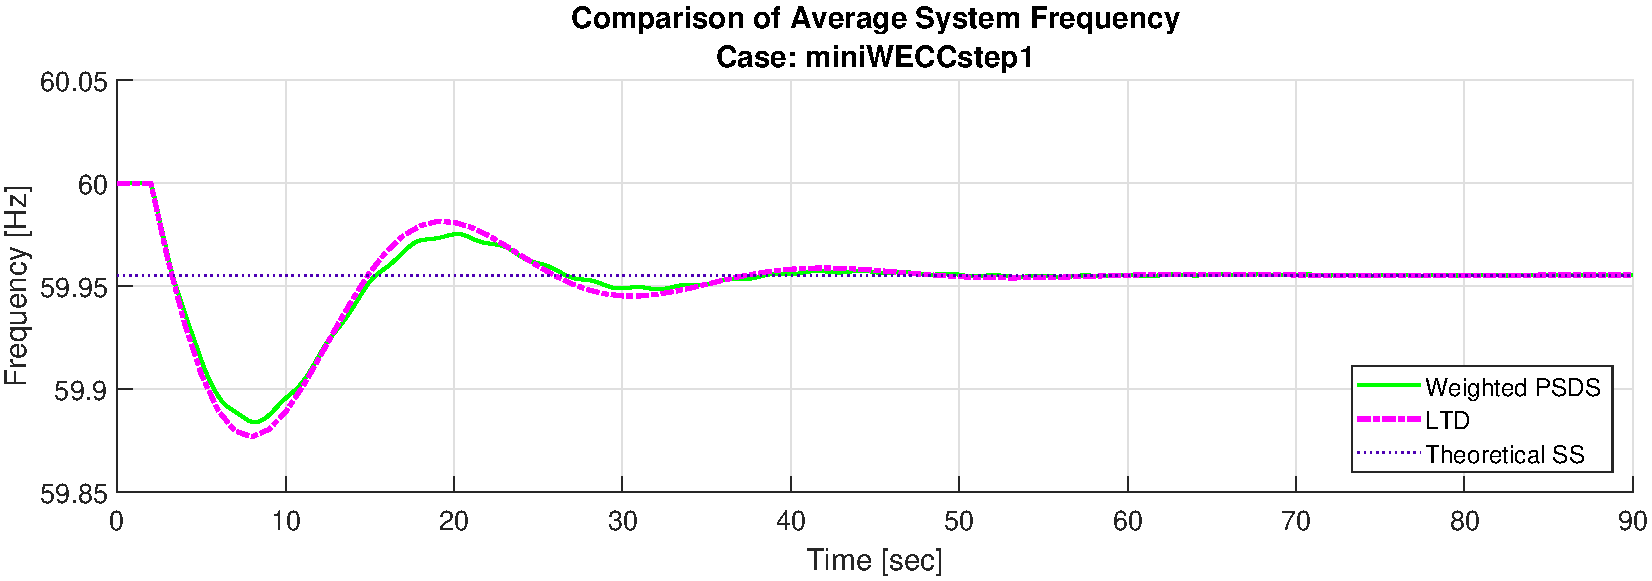
\includegraphics[width=\linewidth]{miniWECCstep1AveF}  \vspace{-2em}
				\caption{Averaged PSDS system response against LTD frequency.} 
				\label{aveF}
	\end{figure}\vspace{-2em}
	\begin{figure}[h!]	
				\centering
				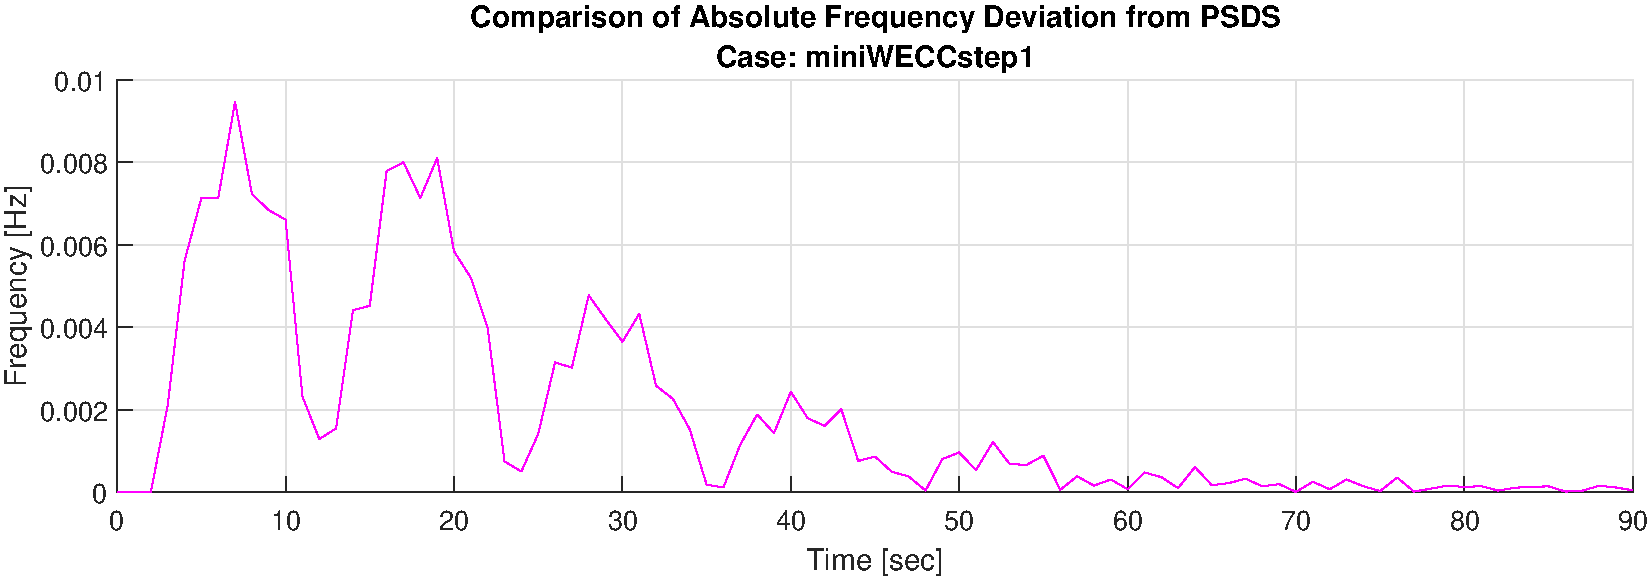
\includegraphics[width=\linewidth]{miniWECCstep1RelF}  \vspace{-1.5em}
				\caption{Relative Hz difference of PSDS - LTD $\left( \text{i.e. }  \left|\dfrac{f_{PSDS}(t)- f_{LTD}(t)}{f_{PSDS}(t)}\right| \times 60 \text{Hz} \right)$.}
				\label{redDif}
	\end{figure}

Improvement from previous results. Load model in dyd changed from \verb|alwscc| with Q as a constant impedance and P as a constant current to \verb|wlwscc| where both P and Q are constant Power.\\
\pagebreak

$P_e$, $P_m$, and $Q$ all match well (reactive power example on last page), however, a number of system voltages don't match at t=0. Additionally, PSDS angles missing (around t= 8, 25, 45, 70) are shifted up near 5 and 6 degrees. Could be an issue with the selected reference bus angle.

	\begin{figure}[h!]
			\centering
			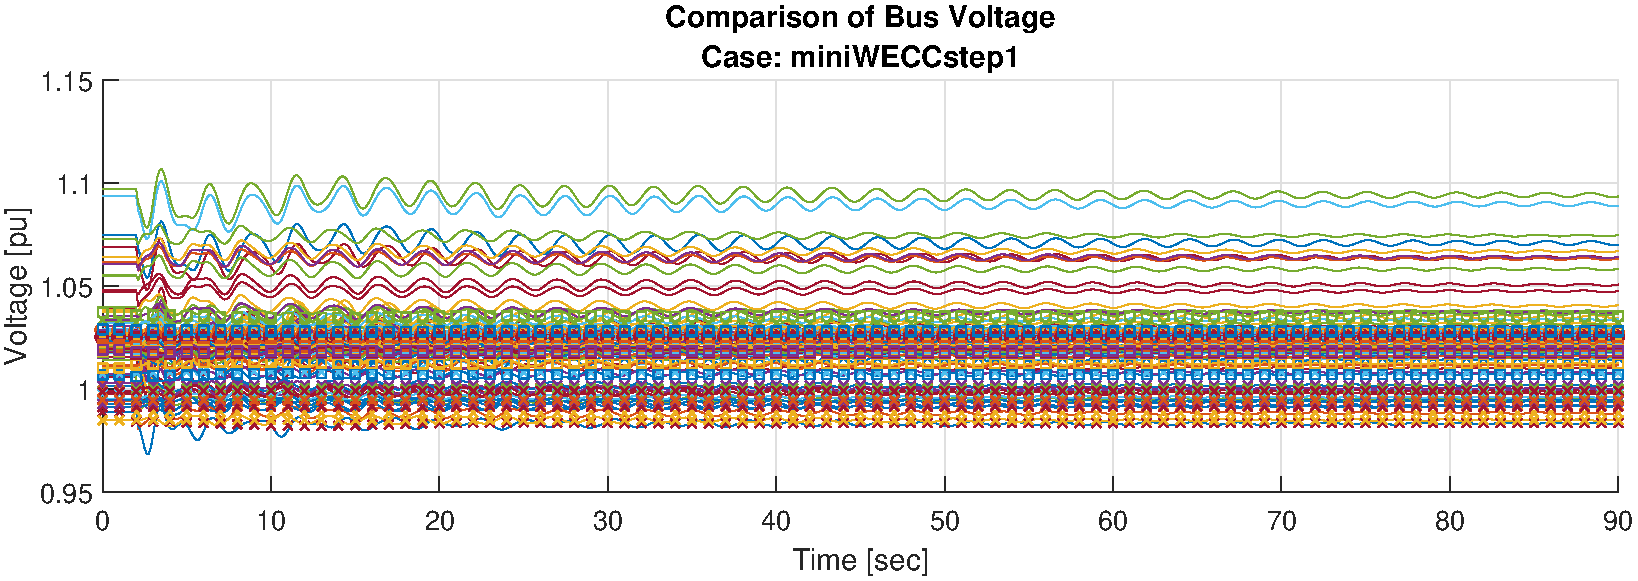
\includegraphics[width=\linewidth]{miniWECCstep1V}\vspace{-1em}
			\caption{Voltage Magnitude Comparison.}
			\label{vMag}		 
	\end{figure}\vspace{-2em}
	\begin{figure}[h!]
				\centering
				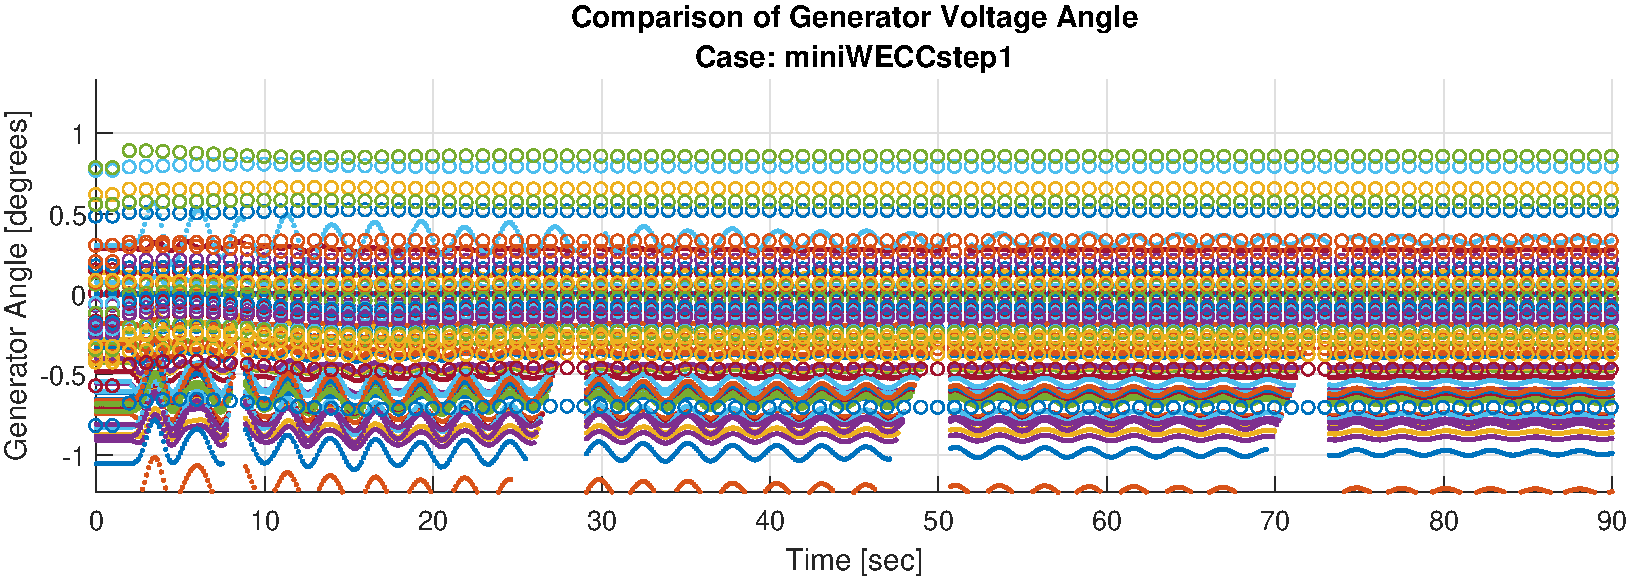
\includegraphics[width=\linewidth]{miniWECCstep1Angle}  \vspace{-2em}
				\caption{Voltage Angle Comparison.} 
				\label{vAng}
	\end{figure}\vspace{-2em}
	\begin{figure}[h!]
				\centering
				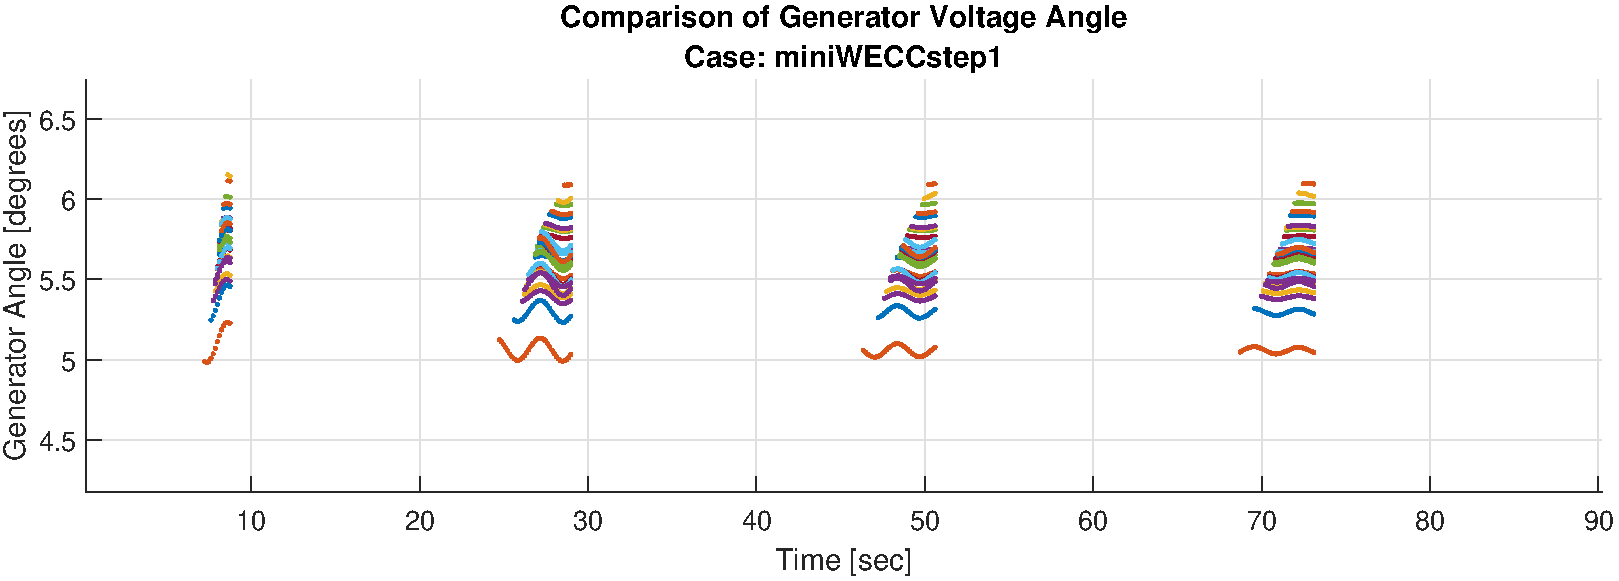
\includegraphics[width=\linewidth]{miniWECCstep1MissingAngle}  \vspace{-2em}
				\caption{Voltage Angle Wrapping.} 
				\label{vAng}
	\end{figure}\vspace{-2em}
\pagebreak


\paragraph{Generator Trip:} Simulation results with time step = 1.0 second. Generator producing 212.5 MW tripped at t=2 (smallest generator in MiniWECC). PSDS must have exciters and PSS models to remain stable. Calculated theoretical SS requires knowing MW tripped and $\Delta P_{losses}$.

\newcommand{\caseName}{miniWECCgenTrip0}
	\begin{figure}[h!]
			\centering
			\includegraphics[width=\linewidth]{\caseName Freq}\vspace{-1em}
			\caption{All PSDS bus frequencies and LTD system frequency response.}
			\label{fcomp}		 
	\end{figure}\vspace{-2em}


	\begin{figure}[h!]
				\centering
				\includegraphics[width=\linewidth]{\caseName AveF}  \vspace{-2em}
				\caption{Averaged PSDS system response against LTD frequency.} 
				\label{aveF}
	\end{figure}\vspace{-2em}
	\begin{figure}[h!]	
				\centering
				\includegraphics[width=\linewidth]{\caseName RelF}  \vspace{-1.5em}
				\caption{Relative Hz difference of PSDS - LTD $\left( \text{i.e. }  \left|\dfrac{f_{PSDS}(t)- f_{LTD}(t)}{f_{PSDS}(t)}\right| \times 60 \text{Hz} \right)$.}
				\label{redDif}
	\end{figure}
Weighted PSDS average frequency adjusted by $\dfrac{H_i M_{BASE_i}}{H_{sys}}$ where the $i$th generator is tripped.

\pagebreak

Again $P_e$, $P_m$, and $Q$ all match well, but a number of system voltages don't match at t=0.

	\begin{figure}[h!]
			\centering
			\includegraphics[width=\linewidth]{\caseName V}\vspace{-1em}
			\caption{Voltage Magnitude Comparison.}
			\label{vMag}		 
	\end{figure}\vspace{-2em}
	\begin{figure}[h!]
				\centering
				\includegraphics[width=\linewidth]{\caseName Angle}  \vspace{-2em}
				\caption{Voltage Angle Comparison.} 
				\label{vAng}
	\end{figure}\vspace{-2em}
	\begin{figure}[h!]
				\centering
				\includegraphics[width=\linewidth]{\caseName MissingAngle}  \vspace{-2em}
				\caption{Voltage Angle Wrapping.} 
				\label{vAng}
	\end{figure}\vspace{-2em}

\pagebreak
\paragraph{Generator Trips that Crash:} Tripping anything but the smallest generator in the miniWECC results in the PSLF load flow not solving. Attempting to trip Colstrip:
\begin{Verbatim}
In IPY redirect...
{'HandoffType': 'PY3toIPY', 'Pacc': -1429.5000000000146, 'msgType': 'Handoff', 
'Pert_Pdelta': 0.0}
* PY3toIPY handoff
prev P load: 105985.000000
current P load: 105985.000000
Pert delta : 0.000000   Pacc -1429.500000
expected: 0.000000       -1429.500000
Perturbance P delta Match
Pacc Match
*** LTD: Distributing -1429.50 MW of Pacc, Iteration 1
Beginning solution
You can interrupt SOLN with <Cntl-c>

It -P-error- --Bus-- ----Name---- --Kv-- area -Q-error- --Bus-- ----Name---- --Kv-- area
   -delta-A- --Bus-- ----Name---- --Kv-- area -delta-V- --Bus-- ----Name---- --Kv-- area

 0   13.8461      32 COLS-GEN      20.00    1  -71.4250      49 SC-49        500.00    1
     87.4744      32 COLS-GEN      20.00    1  0.946379      33 COLSTRP      500.00    1

 1  -93.0123      32 COLS-GEN      20.00    1   51.9179      33 COLSTRP      500.00    1
     97.4184      32 COLS-GEN      20.00    1  0.671771      32 COLS-GEN      20.00    1

 2  334.4607      32 COLS-GEN      20.00    1  143.2892      33 COLSTRP      500.00    1
     17.8952      30 MNT-GEN       20.00    1  1.147258      30 MNT-GEN       20.00    1

 3   87.2405      32 COLS-GEN      20.00    1   37.7330      33 COLSTRP      500.00    1
   8330.6761      76 IDA-76        20.00    1 62.766499      77 IDA-77       230.00    1

Excessive mismatch, aborting iteration

 4  468.0493      77 IDA-77       230.00    1 1163.3152      77 IDA-77       230.00    1
   8330.6761      76 IDA-76        20.00    1 62.766499      77 IDA-77       230.00    1
Stopped on divergence check, CASE NOT SOLVED
Stopped on divergence check, CASE NOT SOLVED
Power Flow Solution returns: -1
*** Error Caught, Simulation Stopping...
*** PSLF power flow solution did not converge.
\end{Verbatim}

\pagebreak

Tripping the 2nd smallest generator in the system (gen on bus 53) hit the maximum iteration count before trying to redistribute remaining $P_{acc}$ and attempting to solve again but not before running into voltage issues. System diverges on 2nd iteration in second attempt at a solution.

\begin{Verbatim}
In IPY redirect...
{'HandoffType': 'PY3toIPY', 'Pacc': -435.00000000001455, 'msgType': 'Handoff', 
'Pert_Pdelta': 0.0}
* PY3toIPY handoff
prev P load: 105985.000000
current P load: 105985.000000
Pert delta : 0.000000   Pacc -435.000000
expected: 0.000000       -435.000000
Perturbance P delta Match
Pacc Match
*** LTD: Distributing -435.00 MW of Pacc, Iteration 1
Beginning solution
You can interrupt SOLN with <Cntl-c>

It -P-error- --Bus-- ----Name---- --Kv-- area -Q-error- --Bus-- ----Name---- --Kv-- area
   -delta-A- --Bus-- ----Name---- --Kv-- area -delta-V- --Bus-- ----Name---- --Kv-- area

 0    4.2633      53 SDG-GEN       20.00    1  -71.4250      49 SC-49        500.00    1
     10.2709      55 SDG-55       110.00    1  0.104277     103 MNT-103      230.00    1

 1   -0.7020      54 SDG-54       500.00    1    1.9695      49 SC-49        500.00    1
      4.7730      55 SDG-55       110.00    1  0.103712      55 SDG-55       110.00    1

 2    1.0767      55 SDG-55       110.00    1    0.1826      55 SDG-55       110.00    1
     82.1392      55 SDG-55       110.00    1  1.748695      55 SDG-55       110.00    1

 3  101.3166      54 SDG-54       500.00    1   52.7344      55 SDG-55       110.00    1
    278.2173      55 SDG-55       110.00    1  2.740665      53 SDG-GEN       20.00    1

 4 -193.2022      54 SDG-54       500.00    1  810.8662      55 SDG-55       110.00    1
     42.3168      52 SC-52        230.00    1  0.547776      55 SDG-55       110.00    1

 5   52.6068      55 SDG-55       110.00    1  200.6331      55 SDG-55       110.00    1
     65.1522      53 SDG-GEN       20.00    1  0.563170      55 SDG-55       110.00    1

 6   30.9338      55 SDG-55       110.00    1   49.5185      55 SDG-55       110.00    1
    149.7914      54 SDG-54       500.00    1  0.870878      54 SDG-54       500.00    1

 7   33.0169      55 SDG-55       110.00    1  -65.0312      57 LASVEGAS     500.00    1
   2880.5991      55 SDG-55       110.00    1 18.117615      54 SDG-54       500.00    1

 8  245.0757      54 SDG-54       500.00    1  223.9316      54 SDG-54       500.00    1
     70.2058      55 SDG-55       110.00    1  0.378723      54 SDG-54       500.00    1

 9   64.5537      54 SDG-54       500.00    1   60.4908      54 SDG-54       500.00    1
     93.5233      55 SDG-55       110.00    1  0.094997      53 SDG-GEN       20.00    1

It -P-error- --Bus-- ----Name---- --Kv-- area -Q-error- --Bus-- ----Name---- --Kv-- area
   -delta-A- --Bus-- ----Name---- --Kv-- area -delta-V- --Bus-- ----Name---- --Kv-- area

10   24.3688      55 SDG-55       110.00    1   17.0381      55 SDG-55       110.00    1
     59.4342      54 SDG-54       500.00    1  0.417368      55 SDG-55       110.00    1

11   17.5804      55 SDG-55       110.00    1    7.8905      61 PV-61        500.00    1
     42.2959      55 SDG-55       110.00    1  0.901168      55 SDG-55       110.00    1

12   22.0870      55 SDG-55       110.00    1   73.4881      63 PHX-63       500.00    1
     16.0814      55 SDG-55       110.00    1  0.148651      55 SDG-55       110.00    1

13   -4.5591      55 SDG-55       110.00    1   17.7221      63 PHX-63       500.00    1
     10.5828      55 SDG-55       110.00    1  0.121005      55 SDG-55       110.00    1

14    3.0140      55 SDG-55       110.00    1    3.0016      63 PHX-63       500.00    1
      5.5029      55 SDG-55       110.00    1  0.130526      55 SDG-55       110.00    1

15    0.8028      55 SDG-55       110.00    1    0.6315      52 SC-52        230.00    1
     75.3235      55 SDG-55       110.00    1  1.607296      55 SDG-55       110.00    1

16   67.6170      54 SDG-54       500.00    1   39.1311      55 SDG-55       110.00    1
    266.4972      55 SDG-55       110.00    1  2.920609      53 SDG-GEN       20.00    1

17 -133.4454      54 SDG-54       500.00    1  558.1630      55 SDG-55       110.00    1
     56.1306      53 SDG-GEN       20.00    1  0.526573      55 SDG-55       110.00    1

18   49.4588      55 SDG-55       110.00    1  138.0932      55 SDG-55       110.00    1
    104.3050      54 SDG-54       500.00    1  0.705451      54 SDG-54       500.00    1

19   32.3658      55 SDG-55       110.00    1   33.1036      55 SDG-55       110.00    1
    452.8957      55 SDG-55       110.00    1  0.716826      55 SDG-55       110.00    1

It -P-error- --Bus-- ----Name---- --Kv-- area -Q-error- --Bus-- ----Name---- --Kv-- area
   -delta-A- --Bus-- ----Name---- --Kv-- area -delta-V- --Bus-- ----Name---- --Kv-- area

20   38.0448      55 SDG-55       110.00    1   16.5559      52 SC-52        230.00    1
    326.6619      54 SDG-54       500.00    1  4.108809      55 SDG-55       110.00    1

21   66.6867      55 SDG-55       110.00    1  137.3597      54 SDG-54       500.00    1
    149.7430      55 SDG-55       110.00    1  1.326245      55 SDG-55       110.00    1

22  118.4120     112 SC-112       110.00    1   47.3383      54 SDG-54       500.00    1
    102.6142      55 SDG-55       110.00    1  5.550318      55 SDG-55       110.00    1

23   28.1265      55 SDG-55       110.00    1  118.6632      57 LASVEGAS     500.00    1
   1342.8722      55 SDG-55       110.00    1  5.420668      53 SDG-GEN       20.00    1

24   35.9450      55 SDG-55       110.00    1   60.8100      52 SC-52        230.00    1
    632.1847      54 SDG-54       500.00    1  4.213779      53 SDG-GEN       20.00    1

25 -312.4132      54 SDG-54       500.00    1  341.8130      55 SDG-55       110.00    1
     92.0843      52 SC-52        230.00    1  0.717109      54 SDG-54       500.00    1

WARNING: SOLUTION stopped due to maximum number of iterations or CONTROL-C hit

Stopped after  26 iterations
Estimated solution error     31241.3203 MW,        34181.3047 MVAR
at buses                  54 SDG-54       500.00      55 SDG-55       110.00 
Power Flow Solution returns: -2
expected: 478.86        actual: 883.03  error: -404.16
*** LTD: Distributing -404.16 MW of Pacc, Iteration 2
Beginning solution
You can interrupt SOLN with <Cntl-c>

Initial voltage magnitude [  0.49] at bus     55 outside of range [0.5, 2.0] p.u
  Resetting it to schedule value of [  1.00]

Initial voltage magnitude [  0.17] at bus     54 outside of range [0.5, 2.0] p.u
  Resetting it to schedule value of [  1.00]

Initial voltage magnitude [  0.29] at bus     53 outside of range [0.5, 2.0] p.u
  Resetting it to schedule value of [  1.02]

It -P-error- --Bus-- ----Name---- --Kv-- area -Q-error- --Bus-- ----Name---- --Kv-- area
   -delta-A- --Bus-- ----Name---- --Kv-- area -delta-V- --Bus-- ----Name---- --Kv-- area

 0  -53.9367      49 SC-49        500.00    1 -347.7013      49 SC-49        500.00    1
    232.9004      55 SDG-55       110.00    1  4.540574      54 SDG-54       500.00    1

Excessive mismatch, aborting iteration

 1 -1029.5880      55 SDG-55       110.00    1 -170.3492      53 SDG-GEN       20.00    1
    232.9004      55 SDG-55       110.00    1  4.540574      54 SDG-54       500.00    1
Stopped on divergence check, CASE NOT SOLVED
Stopped on divergence check, CASE NOT SOLVED
Power Flow Solution returns: -1
*** Error Caught, Simulation Stopping...
*** PSLF power flow solution did not converge.
\end{Verbatim}
\pagebreak
\begin{landscape}
	\begin{figure}[h!]
				\centering
				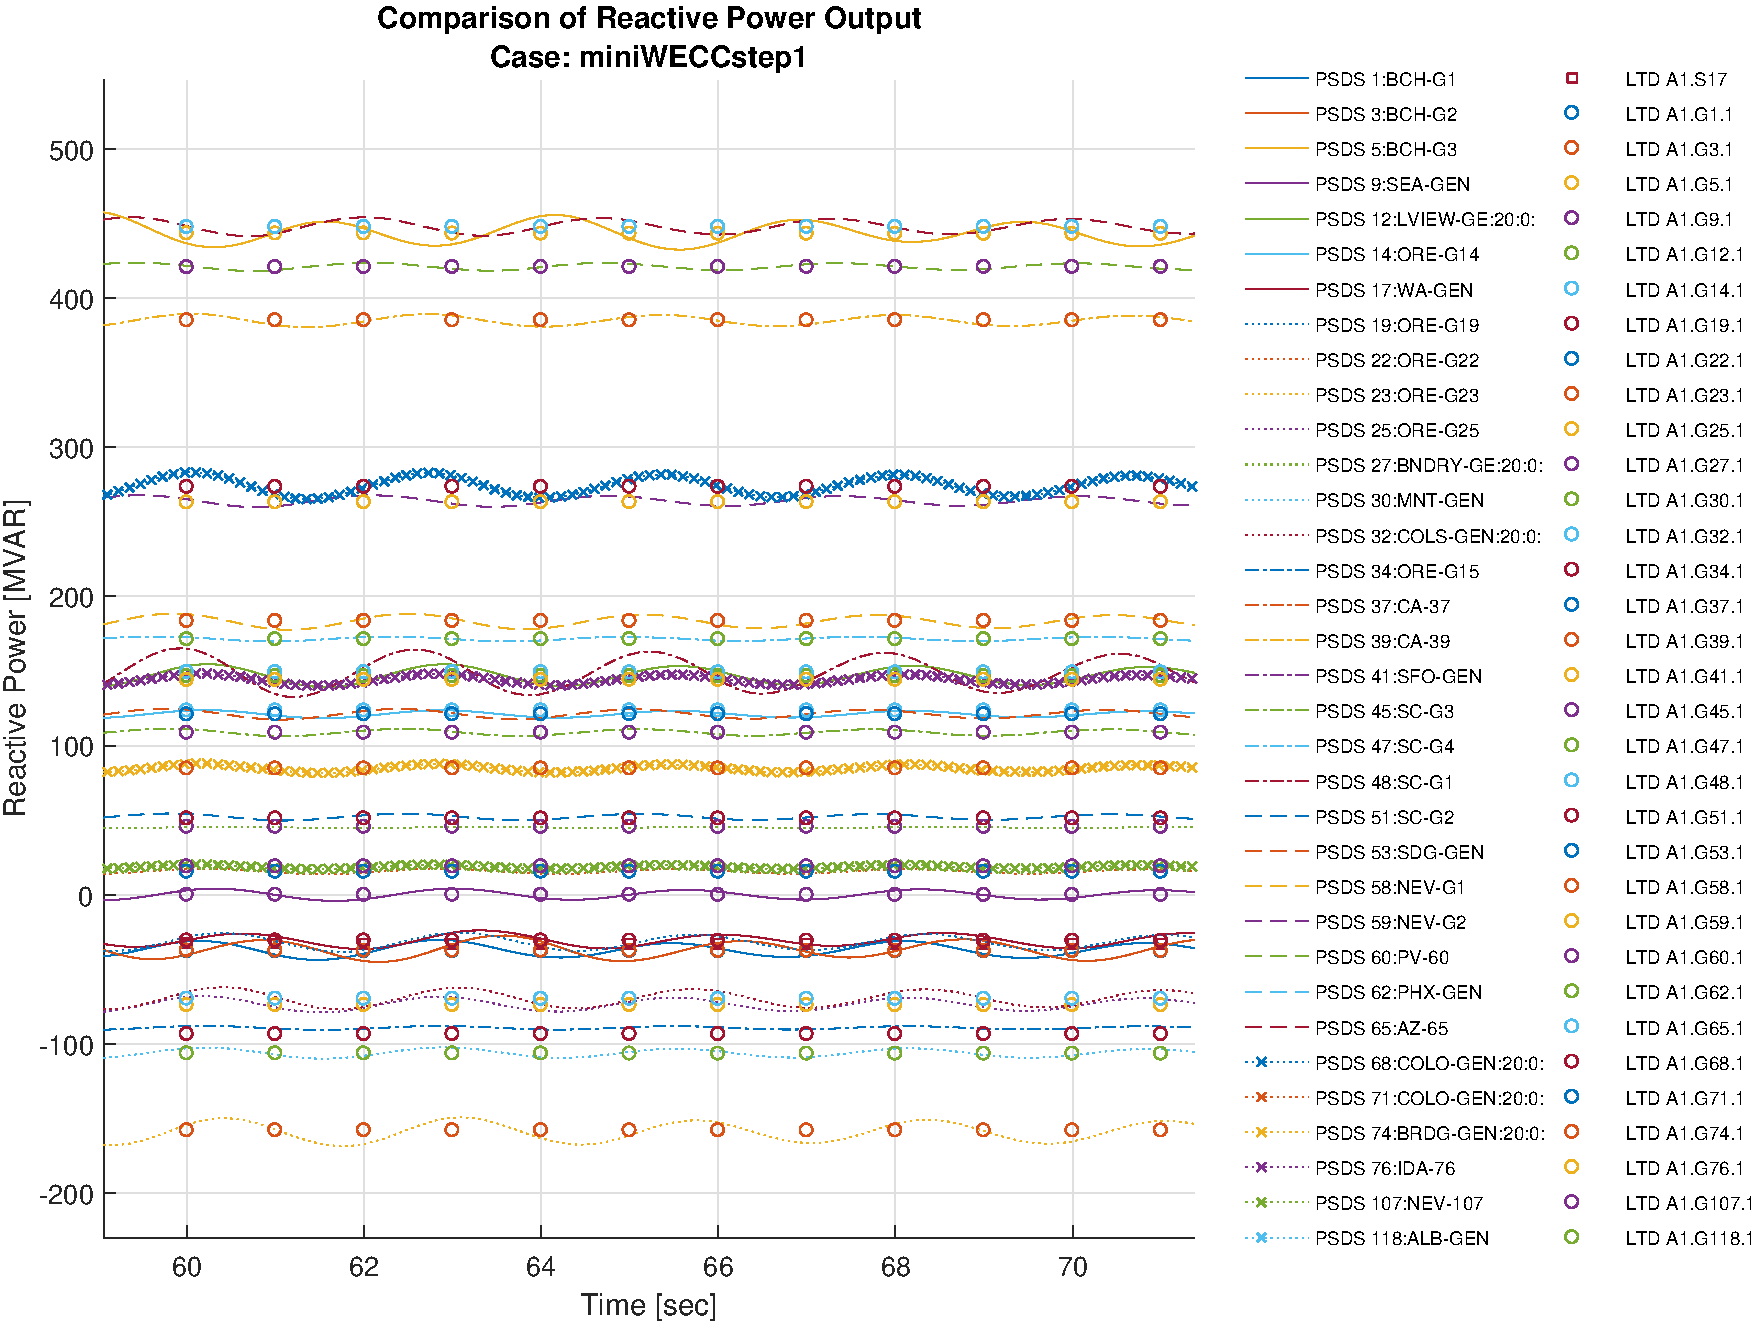
\includegraphics[width=\linewidth]{manyQ}  \vspace{-2em}
				\caption{Detail Recative Power Comparison. Not all Generators shown.} 
				\label{manyQ}
	\end{figure}\vspace{-2em}
\end{landscape}

\end{document}
